% Provenance (never printed): see sources/outline_sources.md (Year 2: ore deposits ---
% magmatic, hydrothermal, sedimentary and supergene deposits; grade and tonnage; exploration).
% Deposit descriptions from the USGS Mineral Deposit Models for Resource Assessment
% (Scientific Investigations Report 2010-5070, chapters A, B, C, E, I, L, N, O, Q), USGS
% Open-File Report 03-077 (orogenic gold) and Grabreck et al. 2022 (kimberlites); the grade and
% tonnage data of the world's porphyry copper deposits from USGS Open-File Report 2008-1155
% (dataset bachelor-2-porphyry-cu). Ledger rows in sources/ledger/book4.md; curves and numbers
% from figdata/bachelor-2/ores.py and the Book 4 second-writer scratch calculator calc/ch29.py.
% Geology and sourced numbers only: no advocacy.
\chapter{Jazidas minerais}\label{ch:b2:ore-deposits}

O cobre constitui cerca de \qty{0.006}{\percent} da crosta; ele é lavrado em rochas que contêm cerca de
\qty{0.5}{\percent}. Toda mina de cobre assenta portanto numa rocha cerca de oitenta vezes mais rica que a
crosta à sua volta, e toda \omterm{def:b2:ore-deposits:deposit}{jazida} é obra de um concentrador natural: um \omterm{def:b2:magma-emplacement:magma}{magma} que
segregou um líquido sulfetado, uma salmoura quente que dissolveu metais e os depositou numa fratura, um
rio que separou grãos pesados de leves, a chuva que lixiviou o topo de um corpo de minério e
redepositou seu cobre mais abaixo. Este capítulo segue esses concentradores, depois mede seus
produtos --- quanto minério, com que \omterm{def:b2:ore-deposits:grade}{teor} --- e termina com a maneira como as \omterm{def:b2:ore-deposits:deposit}{jazidas} são encontradas.
% ledger: perkins:ore-grades

\begin{recall}
\textbf{Dos volumes escolares}: \omterm{def:b2:ore-deposits:deposit}{jazida} e \omterm{def:b2:ore-deposits:cf}{fator de concentração}, veio, \omterm{def:b2:ore-deposits:placer}{placer}, reserva e
recurso; a circulação hidrotermal e as fumarolas negras das dorsais. \textbf{Dos livros de
química}: o minério; a solubilidade, os íons complexos e a oxirredução. \textbf{Do volume do primeiro ano}: a velocidade
de sedimentação de um grão e a lei de Stokes; a laterita; o evaporito. \textbf{Do
\cref{ch:b2:elements-in-the-earth}}: o \omterm{def:b2:elements-in-the-earth:goldschmidt}{elemento calcófilo}, o \omterm{def:b2:elements-in-the-earth:partition}{coeficiente de partição
mineral--fundido}. \textbf{Do \cref{ch:b2:magmatic-differentiation}}: a \omterm{def:b2:magmatic-differentiation:cumulate}{intrusão acamada} e o
\omterm{def:b2:magmatic-differentiation:cumulate}{cumulato}. \textbf{Do \cref{ch:b2:precambrian-earth}}: a \omterm{def:b2:precambrian-earth:bif}{formação ferrífera bandada}, o \omterm{def:b2:precambrian-earth:craton}{cráton}.
\textbf{Dos livros de matemática}: as distribuições normal e lognormal, e a função de
distribuição normal $\Phi$.
\end{recall}

\section{Minério, teor e concentração}\label{sec:b2:ore-deposits:grade}

\begin{definition}[Ganga]\label{def:b2:ore-deposits:ore}
Num minério, a \emph{ganga}\index{ganga} é tudo o que não tem valor econômico: os
minerais formadores de rocha, hidrotermais e de alteração intempérica que acompanham os minerais de minério e são
separados deles e descartados durante o beneficiamento.
\end{definition}

A maior parte do minério é \omterm{def:b2:ore-deposits:ore}{ganga}. Numa \omterm{def:b2:ore-deposits:hydrothermal}{jazida de cobre pórfiro}, a principal fonte mundial de cobre, mais de
\qty{98}{\percent} do minério é \omterm{def:b2:ore-deposits:ore}{ganga}, e os minerais de cobre constituem o resto.
% ledger: usgs10b:share

\begin{definition}[Teor, teor de corte, tonelagem]\label{def:b2:ore-deposits:grade}
O \emph{teor}\index{teor} de um volume de rocha é a fração mássica do elemento ou mineral
valioso que ele contém: em porcentagem para os metais básicos, em gramas por tonelada para o ouro, a prata e os
elementos do grupo da platina. O \emph{teor de corte}\index{teor de corte} é o menor teor com o
qual um bloco de rocha é contado como minério; abaixo dele, o bloco é estéril. A
\emph{tonelagem}\index{tonelagem} de uma \omterm{def:b2:ore-deposits:deposit}{jazida} é a massa de rocha acima do teor de corte; com seu
teor médio $\bar g$ ela dá o metal contido, $M = T\bar g$.
\end{definition}

A \omterm{def:b2:ore-deposits:grade}{tonelagem} e o \omterm{def:b2:ore-deposits:grade}{teor} de uma \omterm{def:b2:ore-deposits:deposit}{jazida} não são, portanto, dois fatos sobre a rocha, mas duas
respostas a uma só pergunta, feita para um dado \omterm{def:b2:ore-deposits:grade}{teor de corte}. Batu Hijau, uma \omterm{def:b2:ore-deposits:deposit}{jazida} de cobre--ouro pórfiro na
Indonésia, é declarada com \qty{914}{Mt} a \qty{0.53}{\percent} de cobre acima de um
\omterm{def:b2:ore-deposits:grade}{teor de corte} de \qty{0.3}{\percent}, e com \qty{1640}{Mt} a \qty{0.44}{\percent} numa compilação mundial
que adota o menor \omterm{def:b2:ore-deposits:grade}{teor de corte} disponível: baixar o \omterm{def:b2:ore-deposits:grade}{teor de corte} quase dobra a \omterm{def:b2:ore-deposits:grade}{tonelagem} e
reduz o \omterm{def:b2:ore-deposits:grade}{teor} médio. Numa \omterm{def:b2:ore-deposits:deposit}{jazida} sedimentar de zinco--chumbo, a \omterm{def:b2:ore-deposits:deposit}{jazida} de Tom no Canadá, uma redução
do \omterm{def:b2:ore-deposits:grade}{teor de corte} de cerca de um por cento de zinco mais chumbo multiplicaria as reservas por cinco.
% ledger: usgs10b:cutoffs, usgs08:tonnage-def, usgs10n:sedex

\begin{definition}[Fator de concentração]\label{def:b2:ore-deposits:cf}
O \emph{fator de concentração}\index{fator de concentração} de um elemento num minério é a razão
$\mathrm{CF} = g/a$ entre seu \omterm{def:b2:ore-deposits:grade}{teor} $g$ e sua abundância $a$ num reservatório de referência, indicado junto:
a crosta continental inteira, a crosta continental superior, ou a rocha a partir da qual a \omterm{def:b2:ore-deposits:deposit}{jazida} se formou.
\end{definition}

O fator depende da referência. Tomando \qty{0.006}{\percent} de cobre para a crosta e
\qty{0.5}{\percent} para o minério, obtém-se um fator de 83; tomando a crosta continental superior,
\qty{28}{ppm}, e o \omterm{def:b2:ore-deposits:grade}{teor} médio dos cobres pórfiros de 2008, \qty{0.44}{\percent}, obtém-se 157. O ouro,
a \qty{1.5}{ng/g} na crosta superior e lavrado a alguns gramas por tonelada, tem fatores da ordem dos
milhares; o ferro, a vários por cento na crosta e lavrado a cerca de \qty{50}{\percent}, precisa
de um fator de apenas cerca de dez.
% ledger: perkins:ore-grades, rg03:ucc-trace, usgs10b:share, earle:ore-grades, earle:iron-grade

\begin{definition}[Jazida]\label{def:b2:ore-deposits:deposit}
Uma \emph{jazida}\index{jazida} é um corpo de rocha no qual processos naturais
concentraram um elemento ou um mineral a um \omterm{def:b2:ore-deposits:grade}{teor} acima do \omterm{def:b2:ore-deposits:grade}{teor de corte}, numa \omterm{def:b2:ore-deposits:grade}{tonelagem} grande o bastante
para que seja extraído com lucro. É ao mesmo tempo um objeto geológico, definido pelos processos que
o formaram, e um objeto econômico, definido pelos preços, pelos custos e pela tecnologia.
\end{definition}

Por causa de sua metade econômica, o tamanho de uma \omterm{def:b2:ore-deposits:deposit}{jazida} muda com o tempo. Os recursos identificados
de um elemento são as concentrações das quais a extração é viável hoje ou pode vir a sê-lo; suas
reservas são a parte que poderia ser extraída economicamente no momento em que foram determinadas. As reservas mundiais
de cobre eram de \qty{280}{Mt} em 1970; cerca de \qty{697}{Mt} foram lavradas desde então, e elas
eram de \qty{980}{Mt} em 2024.
% ledger: usgs:mcs-reserves

\begin{proposition}[Balanço de massa de uma jazida]\label{prop:b2:ore-deposits:mass-balance}
Uma \omterm{def:b2:ore-deposits:deposit}{jazida} que contém uma massa $M$ de um elemento com \omterm{def:b2:ore-deposits:grade}{teor} médio $g$ foi alimentada por uma fonte na qual o
elemento tinha abundância $a$. Se o processo concentrador extraiu uma fração $\eta \leq 1$ do
elemento da fonte e a entregou à \omterm{def:b2:ore-deposits:deposit}{jazida}, a massa de rocha-fonte processada foi
\begin{equation}
m_{\mathrm{source}} = \frac{M}{\eta\,a} = \frac{\mathrm{CF}}{\eta}\, T ,
\label{eq:b2:ore-deposits:mass-balance}
\end{equation}
com $T = M/g$ a \omterm{def:b2:ore-deposits:grade}{tonelagem} e $\mathrm{CF} = g/a$: pelo menos CF toneladas de fonte por tonelada de minério.
\end{proposition}

\begin{proof}
A fonte perdeu $\eta\,a\,m_{\mathrm{source}}$ do elemento e a \omterm{def:b2:ore-deposits:deposit}{jazida} recebeu $M$; igualando
as duas obtém-se a primeira forma, e $M = gT$ dá a segunda. Como $\eta \leq 1$, $m_{\mathrm{source}} \geq
\mathrm{CF}\,T$.
\end{proof}

Bingham Canyon, a \omterm{def:b2:ore-deposits:deposit}{jazida} pórfira mostrada abaixo, é listada com \qty{3230}{Mt} a
\qty{0.882}{\percent} de cobre, \qty{28.5}{Mt} de cobre. Seu fator em relação à crosta superior é 315,
e mesmo um processo perfeitamente eficiente teria tido de drenar \num{1.02e12} toneladas de crosta
superior média, cerca de \qty{377}{km^3}: um cubo de \qty{7.2}{km} de lado. Os processos formadores de minério são
portanto processos que movem muita matéria --- \omterm{def:b2:magma-emplacement:magma}{magma}, água, sedimento --- através de um pequeno
volume onde o elemento fica retido.
% ledger: data:b4-porphyry-cu, rg03:ucc-trace
% values: 28.49 Mt; CF 315; 1.0175e12 t; 377 km3 at 2.7 t/m3; side 7.22 km (calc/ch29.py)

\begin{omfigure}
\centering
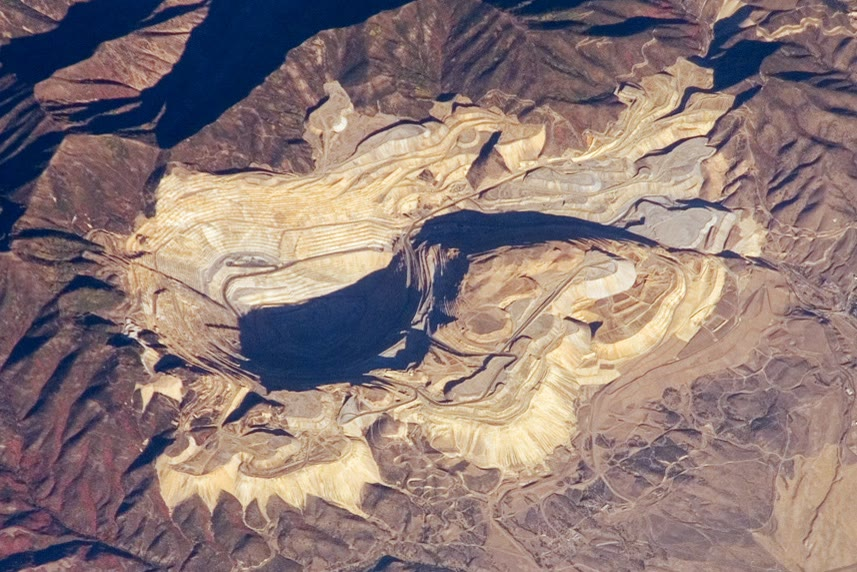
\includegraphics[width=0.5\linewidth]{images/book4/b2-29-bingham-canyon-iss.jpg}
\par\smallskip{\small A cava a céu aberto de Bingham Canyon, Utah, vista da Estação Espacial Internacional
(2007): mais de \qty{4}{km} de largura e \qty{1200}{m} de profundidade, escavada em bancadas de 16 a \qty{25}{m} de altura
numa \omterm{def:b2:ore-deposits:hydrothermal}{jazida de cobre pórfiro}; as colinas de topo plano à sua volta são pilhas de estéril. Fotografia:
NASA, tripulação da Expedição 15 (domínio público).}
\end{omfigure}
% ledger: photo:b2-29-bingham

\begin{definition}[Tipos de jazida]\label{def:b2:ore-deposits:types}
Um \emph{tipo de jazida}\index{tipo de jazida} é uma classe de \omterm{def:b2:ore-deposits:deposit}{jazidas} que compartilham um contexto
geológico, uma rocha encaixante, uma forma, uma mineralogia de minério e um processo de formação, de modo que uma descrição da
classe prevê onde seus membros ocorrem. Os tipos dividem-se em quatro famílias segundo o processo:
magmáticas (o metal é concentrado por um \omterm{def:b2:magma-emplacement:magma}{magma} enquanto ele cristaliza ou se segrega),
hidrotermais (por um fluido aquoso quente), sedimentares (pelo transporte e pela deposição
de sedimento, ou por precipitação a partir da água na superfície), e supergênicas (pelo intemperismo
de uma \omterm{def:b2:ore-deposits:deposit}{jazida} anterior).
\end{definition}

\section{Jazidas magmáticas}\label{sec:b2:ore-deposits:magmatic}

\textbf{A cromita nas intrusões acamadas.} A cromita, a única fonte comercial de cromo,
acumula-se em camadas de cromitito maciço, com mais de \qty{90}{\percent} de cromita, nas partes inferiores
ultramáficas das intrusões acamadas. As intrusões têm de 2 a \qty{180}{km} de diâmetro e até
\qty{15}{km} de espessura, e as camadas vão de menos de um centímetro a 5--\qty{8}{m}; juntas
elas contêm a maior parte das reservas mundiais de cromo, e o Complexo de Bushveld, encontrado no
\cref{ch:b2:magmatic-differentiation}, é o único lavrado para cromita hoje. Sua origem, uma
camada de \omterm{def:b2:magmatic-differentiation:cumulate}{cumulato} forçada para o campo da cromita pela \omterm{def:b2:magmatic-differentiation:open}{mistura de magmas} ou por uma mudança de pressão ou
de estado de oxidação, ainda é debatida.
% ledger: usgs10e:chromite

\textbf{Sulfetos de níquel--cobre--EGP.} Um \omterm{def:b2:magma-emplacement:magma}{magma} máfico ou ultramáfico, produzido por grandes graus de
fusão do manto (\qty{20}{\percent} a \qty{25}{\percent} ou mais, com mais de 12 por cento de MgO em
massa), sobe subsaturado em enxofre. Se assimila enxofre da crosta, ou se resfria o
bastante, torna-se saturado e um líquido sulfetado imiscível separa-se em gotículas. Os
metais calcófilos passam para essas gotículas: a razão $D$ entre sua concentração no líquido
sulfetado e no líquido silicático, o mesmo tipo de coeficiente de partição que entre um
mineral e um líquido, é de $10^2$ a $10^3$ para o cobre e o níquel e de $10^3$ a $10^4$ para os
elementos do grupo da platina. Quanto metal uma gotícula recolhe depende então de quanto \omterm{def:b2:magma-emplacement:magma}{magma} ela encontra.
% ledger: usgs10i:r-factor

\begin{proposition}[Fator R]\label{prop:b2:ore-deposits:r-factor}
Suponha-se que uma massa unitária de líquido sulfetado se separe de uma massa $R$ de \omterm{def:b2:magma-emplacement:magma}{magma} silicático, e atinja o equilíbrio com ela
(essa massa é o \emph{fator R}\index{fator R}), num sistema fechado; seja $C_L$ a concentração de um
metal no \omterm{def:b2:magma-emplacement:magma}{magma} antes da separação do sulfeto, e $D$ seu coeficiente de partição
sulfeto--silicato. Então a concentração do metal no sulfeto é
\begin{equation}
C_S = C_L\,\frac{D\,(R + 1)}{R + D} .
\label{eq:b2:ore-deposits:r-factor}
\end{equation}
Para $R \gg D$, $C_S \to D\,C_L$; para $R \ll D$, $C_S \approx (R + 1)\,C_L$.
\end{proposition}

\begin{proof}
O sistema de massa $R + 1$ continha $(R + 1)C_L$ do metal antes da separação. Depois dela, o silicato
contém $R\,C_{\mathrm{sil}}$ e o sulfeto $C_S$, com $C_S = D\,C_{\mathrm{sil}}$ no equilíbrio.
A conservação dá $(R + 1)C_L = R\,C_S/D + C_S = C_S\,(R + D)/D$, donde
\eqref{eq:b2:ore-deposits:r-factor}. Se $R \gg D$, $(R + 1)/(R + D) \to 1$; se $R \ll D$,
$D/(R + D) \to 1$.
\end{proof}

Os dois limites explicam por que existem dois tipos de minério sulfetado. Quando $R \ll D$ o sulfeto toma
quase todo o metal do \omterm{def:b2:magma-emplacement:magma}{magma} que encontra e $C_S$ cresce com $R$; quando $R \gg D$ ele fica
saturado em $D\,C_L$ e mais \omterm{def:b2:magma-emplacement:magma}{magma} não acrescenta nada. O níquel e o cobre, com $D$ de algumas centenas,
atingem seu teto com $R$ de algumas centenas a alguns milhares, a faixa da maioria dos minérios de níquel--cobre;
a platina e o paládio, com $D$ perto de $10^4$, continuam ganhando até $R$ de \num{10000} a
\num{100000}. Os minérios ricos em elementos do grupo da platina, como o Merensky Reef do Bushveld e
alguns minérios de Norilsk, registram portanto uma pequena massa de sulfeto lavada por uma massa muito grande de
\omterm{def:b2:magma-emplacement:magma}{magma} (exercícios~\ref{exo:b2:ore-deposits:5} e~\ref{exo:b2:ore-deposits:11}).
% ledger: usgs10i:r-factor

\textbf{Kimberlitos e diamantes.} A maioria dos diamantes, e quase todos os lavrados, formou-se na base da
litosfera continental espessa, nas raízes dos \omterm{def:b2:precambrian-earth:craton}{crátons}; os \omterm{def:b2:magma-emplacement:magma}{magmas} kimberlíticos, vindos de profundidades
maiores que 120 a \qty{150}{km} e subindo a até \qty{20}{m.s^{-1}}, levam-nos à
superfície depressa o bastante para que sobrevivam. Os kimberlitos irrompem preferencialmente através de litosfera espessa e antiga,
que é onde a prospecção de diamantes procura.
% ledger: grabreck22:kimberlite

\textbf{Pegmatitos.} Os pegmatitos de lítio--césio--tântalo são \omterm{def:b2:magma-emplacement:bodies}{diques} graníticos enriquecidos nesses elementos
raros, produzidos em \omterm{def:b2:alpine-orogen:orogen}{orógenos} colisionais; cristalizam a cerca de 350 a \qty{550}{\celsius},
temperatura notavelmente baixa para um líquido granítico, em dias a anos, e formam cristais enormes --- um
cristal de espodumênio media \qty{14}{m} de comprimento. Seus minerais de lítio, espodumênio, petalita e
lepidolita, fornecem cerca de um quarto do lítio mundial.
% ledger: usgs10o:lct

\section{Jazidas hidrotermais}\label{sec:b2:ore-deposits:hydrothermal}

\begin{definition}[Fluido hidrotermal e tipos de jazidas hidrotermais]\label{def:b2:ore-deposits:hydrothermal}
Um \emph{fluido hidrotermal}\index{fluido hidrotermal} é um fluido aquoso quente, liberado por um \omterm{def:b2:magma-emplacement:magma}{magma},
por \omterm{def:b2:metamorphic-facies:reaction}{reações metamórficas}, ou água do mar, água meteórica ou salmoura de bacia aquecidas, que dissolve,
transporta e deposita elementos ao fluir através da rocha. Os principais \omterm{def:b2:ore-deposits:types}{tipos de jazidas} hidrotermais
são:
\begin{itemize}
  \item a \emph{jazida de cobre pórfiro}\index{jazida de cobre pórfiro}: um corpo grande, de baixo \omterm{def:b2:ore-deposits:grade}{teor},
        de vênulas e sulfetos de cobre disseminados dentro e em torno de um pequeno stock pórfiro, formado por
        fluidos magmáticos a poucos quilômetros da superfície acima de uma zona de subducção;
  \item a \emph{jazida epitermal}\index{jazida epitermal}: veios e
        disseminações de ouro--prata formados a menos de cerca de \qty{1.5}{km} da superfície, a cerca de 100 a
        \qty{300}{\celsius}, em arcos vulcânicos;
  \item a \emph{jazida de sulfeto maciço vulcanogênico}\index{jazida de sulfeto maciço vulcanogênico}
        (VMS): uma lente de sulfetos maciços formada sobre o fundo do mar ou logo abaixo dele, numa fonte
        hidrotermal num contexto vulcânico submarino;
  \item a \emph{jazida sedimentar exalativa}\index{jazida sedimentar exalativa} (sedex):
        sulfetos laminados de zinco--chumbo em folhelhos marinhos de uma \omterm{def:b2:basins-compared:types}{bacia de rifte}, precipitados sobre o fundo do mar ou logo
        abaixo dele a partir de salmouras de bacia que sobem ao longo de falhas;
  \item a \emph{jazida do tipo Mississippi Valley}\index{jazida do tipo Mississippi Valley} (MVT):
        sulfetos de zinco--chumbo que substituem carbonatos de plataforma, epigenéticos e sem relação com atividade
        ígnea, depositados por salmouras de bacia;
  \item a \emph{jazida de ouro orogênico}\index{jazida de ouro orogênico}: veios de quartzo aurífero em
        cinturões metamórficos, ao longo de grandes falhas, depositados por fluidos de baixa salinidade, ricos em CO$_2$, de
        origem metamórfica.
\end{itemize}
\end{definition}
% ledger: usgs10b:form, usgs10q:epithermal, usgs10c:vms, usgs10n:sedex, usgs10a:mvt, drew03:orogenic

\textbf{Transporte e deposição.} A maioria dos metais é transportada nos fluidos hidrotermais como complexos:
o zinco, o chumbo e o cobre como clorocomplexos, de modo que a salinidade controla sua solubilidade, e o ouro,
em fluidos reduzidos, como complexos de enxofre como AuHS(H$_2$S)$_3$. Um fluido deposita sua carga quando a
solubilidade cai: quando ele se resfria; quando ferve com a queda de sua pressão, perdendo H$_2$S e CO$_2$ e
mudando o pH; quando se mistura com um fluido de composição diferente --- uma salmoura que encontra água rica
em H$_2$S precipita esfalerita e galena quase de imediato; e quando reage com a rocha
encaixante, o que muda seu pH ou seu estado de oxidação. Cada \omterm{def:b2:ore-deposits:types}{tipo de jazida} é uma combinação de fluido,
caminho e armadilha.
% ledger: usgs10n:sedex, drew03:orogenic

\textbf{Cobre pórfiro.} As \omterm{def:b2:ore-deposits:deposit}{jazidas} pórfiras fornecem cerca de \qty{60}{\percent} do cobre
mundial e contêm cerca de \qty{65}{\percent} de seus recursos. Elas se centram em pequenos stocks
cilíndricos ou enxames de \omterm{def:b2:magma-emplacement:bodies}{diques}, os topos de \omterm{def:b2:magma-emplacement:bodies}{plútons} maiores, alojados a menos de 5--\qty{10}{km} de profundidade em
arcos acima de zonas de subducção, o contexto do \cref{ch:b2:magmatic-series}. Uma \omterm{def:b2:ore-deposits:deposit}{jazida} tem de 0.1 a
\qty{1}{km} de diâmetro, com altura semelhante; a rocha alterada pode estender-se por \qty{10}{km} ou mais à sua volta.
À medida que o \omterm{def:b2:magma-emplacement:magma}{magma} cristaliza, um fluido com 3 a 5 por cento de sal em massa separa-se dele; subindo e
descomprimindo-se, divide-se numa salmoura e num vapor, ambos portadores de metais, e sua sobrepressão
fratura a rocha. Veios de quartzo precipitam a cerca de 700 a \qty{500}{\celsius}, e a
reação do fluido com a rocha zoneia a alteração, como no corte abaixo. Como se
formam rasas em margens ativas, onde a erosão é rápida, mais de \qty{90}{\percent} das \omterm{def:b2:ore-deposits:deposit}{jazidas} pórfiras
conhecidas são cenozoicas ou mesozoicas.
% ledger: usgs10b:share, usgs10b:form, usgs10b:fluids, usgs10b:alteration

\begin{omfigure}
\centering
\begin{tikzpicture}[x=1.15cm, y=1.15cm, font=\small]
\begin{scope}
\clip (-2.9,-3.6) rectangle (2.9,0);
% propylitic halo
\fill[omLithBasalt!45] (0,-1.25) ellipse (2.45 and 1.55);
% sodic-calcic deep flanks
\fill[omExo!25] (-1.75,-2.55) ellipse (0.45 and 0.38);
\fill[omExo!25] (1.75,-2.55) ellipse (0.45 and 0.38);
% sericitic shell
\fill[yellow!35] (0,-1.05) ellipse (1.15 and 1.15);
% potassic core
\fill[omProp!40] (0,-1.45) ellipse (0.68 and 0.85);
% ore shell
\draw[omThm, line width=1.1pt, densely dashed] (0,-1.3) ellipse (0.92 and 0.98);
% advanced argillic lithocap
\fill[omDef!30] (-1.05,0) .. controls (-0.6,-0.5) and (0.6,-0.5) .. (1.05,0) -- cycle;
\draw[omDef!70] (-1.05,0) .. controls (-0.6,-0.5) and (0.6,-0.5) .. (1.05,0);
\end{scope}
% pluton and stock
\fill[omLithGranite] (-2.6,-3.6) .. controls (-2.2,-2.9) and (-0.9,-2.6) .. (-0.3,-2.6)
  -- (-0.3,-1.25) arc[start angle=180, end angle=0, radius=0.3] -- (0.3,-2.6)
  .. controls (0.9,-2.6) and (2.2,-2.9) .. (2.6,-3.6) -- cycle;
\draw[black!60] (-2.6,-3.6) .. controls (-2.2,-2.9) and (-0.9,-2.6) .. (-0.3,-2.6)
  -- (-0.3,-1.25) arc[start angle=180, end angle=0, radius=0.3] -- (0.3,-2.6)
  .. controls (0.9,-2.6) and (2.2,-2.9) .. (2.6,-3.6);
% epithermal veins
\foreach \x in {1.45,1.65,1.85} \draw[omDef, line width=1pt] (\x,-0.02) -- (\x+0.12,-0.7);
% palaeosurface
\draw[black, line width=0.8pt] (-2.9,0) -- (2.9,0);
\node[anchor=south west, font=\scriptsize] at (-2.9,0) {paleossuperfície};
% labels
\draw[black!50] (0.6,-0.15) -- (1.2,0.25) -- (3.0,0.25) node[anchor=west, text=black] {argílica avançada};
\draw[black!50] (1.95,-0.3) -- (3.0,-0.3) node[anchor=west, text=black] {veios epitermais};
\draw[black!50] (1.05,-0.8) -- (3.0,-0.8) node[anchor=west, text=black] {sericítica};
\draw[black!50] (0.85,-1.25) -- (3.0,-1.25) node[anchor=west, text=omThm] {casca de minério de cobre};
\draw[black!50] (0.45,-1.7) -- (3.0,-1.7) node[anchor=west, text=black] {potássica};
\draw[black!50] (1.05,-2.15) -- (3.0,-2.15) node[anchor=west, text=black] {propilítica};
\draw[black!50] (2.1,-2.6) -- (3.0,-2.6) node[anchor=west, text=black] {sódico-cálcica};
\draw[black!50] (1.5,-3.15) -- (3.0,-3.15) node[anchor=west, text=black] {plúton e stock pórfiro};
\end{tikzpicture}
\par\smallskip{\small Um sistema de cobre pórfiro em corte (um desenho, sem escala): a zona potássica
no núcleo, profunda e quente; a zona sericítica para cima e para fora, onde a pirita é
abundante; a casca de minério de cobre entre elas; o halo propilítico a profundidades rasas a moderadas
em volta; a alteração sódico-cálcica nos flancos profundos; um capeamento argílico avançado e, em alguns
sistemas, veios epitermais perto da superfície.}
\end{omfigure}
% ledger: usgs10b:alteration

\textbf{Ouro epitermal.} Acima de alguns sistemas pórfiros, e nos arcos vulcânicos em geral, o mesmo
tipo de fluido atinge os \qty{1.5}{km} superiores da crosta a cerca de 100 a \qty{300}{\celsius},
onde ferve e se mistura com a água subterrânea; ele deposita ouro e prata em veios de quartzo, com uma
alteração que registra fluidos quase neutros (adulária, illita) ou muito ácidos (caulinita,
dickita, pirofilita).
% ledger: usgs10q:epithermal, usgs10q:alteration

\textbf{Sulfetos maciços no fundo do mar.} A água do mar aspirada para a crosta quente de uma dorsal ou de
um arco retorna nas fontes como fumarolas negras a cerca de \qty{350}{\celsius}, vistas pela primeira vez na Dorsal do Pacífico
Leste em 1979. Onde o campo de fontes perdura, seus sulfetos constroem um monte; o minério tem mais de
\qty{40}{\percent} de sulfetos, sobre um stockwork de veios que marca o conduto alimentador. Os metais são zoneados
pela temperatura, ferro e cobre na base quente, zinco, ferro, chumbo e bário no topo e nas
margens mais frias, como no monte desenhado na próxima seção. As \omterm{def:b2:ore-deposits:hydrothermal}{jazidas de sulfeto maciço vulcanogênico}
vão de bolsões de menos de uma tonelada aos \qty{1.5}{Gt} de Rio Tinto na Espanha, e em
idade de \qty{3.55}{\Ga} a \omterm{def:b2:ore-deposits:deposit}{jazidas} que se formam hoje.
% ledger: usgs10c:vms

\textbf{Salmouras de bacia: sedex e MVT.} As salmouras de bacia com 10 a \qty{30}{\percent} de sais dissolvidos,
aquecidas a 100--\qty{200}{\celsius} pelo soterramento, transportam zinco e chumbo como clorocomplexos e formam os
dois tipos hospedados em sedimentos. As \omterm{def:b2:ore-deposits:deposit}{jazidas} sedex formam-se onde a salmoura sai numa bacia restrita e redutora
ao longo de uma falha de rifte e encontra sulfeto de hidrogênio, produzindo lamas sulfetadas laminadas; elas contêm mais
da metade das reservas mundiais de zinco e chumbo. As \omterm{def:b2:ore-deposits:deposit}{jazidas} MVT formam-se onde a salmoura, expulsa de uma
bacia, atinge uma plataforma carbonática em sua margem e a substitui a 75 a cerca de
\qty{200}{\celsius}; elas contêm \qty{38}{\percent} do chumbo e do zinco das \omterm{def:b2:ore-deposits:deposit}{jazidas} hospedadas em sedimentos,
com cerca de dez vezes mais zinco que chumbo.
% ledger: usgs10n:sedex, usgs10a:mvt

\textbf{Ouro orogênico.} Nos cinturões metamórficos, \omterm{def:b2:metamorphic-facies:reaction}{reações de desvolatilização} liberam um fluido quase neutro,
de baixa salinidade e rico em CO$_2$; canalizado ao longo de grandes falhas, ele deposita veios de quartzo
auríferos a cerca de \qty{350}{\celsius} e 4 a \qty{12}{km} de profundidade. Os veios são contínuos ao longo de
grandes alturas: \qty{3.2}{km} em Kolar, na Índia.
% ledger: drew03:orogenic

\section{Jazidas sedimentares e supergênicas}\label{sec:b2:ore-deposits:sedimentary}

\begin{definition}[Depósito de placer]\label{def:b2:ore-deposits:placer}
Um \emph{placer}\index{placer} é uma \omterm{def:b2:ore-deposits:deposit}{jazida} sedimentar de minerais densos e duráveis concentrados pela
água ou pelo vento em movimento porque, para o mesmo tamanho, eles sedimentam mais depressa e são arrastados com menos facilidade
que os grãos de quartzo à sua volta.
\end{definition}

Os minerais com densidade acima de cerca de 2.85 são chamados pesados, contra 2.65 para o quartzo: ilmenita e zircão
perto de 4.7, magnetita 5.2, ouro 15 a 19.3. Pela lei de Stokes a velocidade de sedimentação de um grão cresce com
seu excesso de densidade $\rho_s - \rho_w$, onze vezes maior para o ouro que para o quartzo, de modo que o ouro de um
dado tamanho fica junto com quartzo três vezes maior (exercício~\ref{exo:b2:ore-deposits:3}); o ouro
fica em geral nos cascalhos fluviais sobre o embasamento, enquanto a ilmenita, o rutilo e o zircão chegam às praias e às
dunas. Os \omterm{def:b2:ore-deposits:grade}{teores} das areias de minerais pesados são a porcentagem em massa de minerais pesados.
% ledger: usgs10l:heavy, usgs:gold-placer

Os sedimentos químicos também são minérios. As \omterm{def:b2:precambrian-earth:bif}{formações ferríferas bandadas} do \cref{ch:b2:precambrian-earth},
precipitadas quando o ferro dissolvido dos oceanos foi oxidado, são um minério de ferro comum; os evaporitos
fornecem a halita e os sais de potássio; as lateritas, resíduo do intemperismo tropical profundo,
concentram o alumínio como bauxita. O intemperismo também enriquece \omterm{def:b2:ore-deposits:deposit}{jazidas} anteriores.
% ledger: earle:bif, usgs:bauxite

\begin{definition}[Enriquecimento supergênico, gossan]\label{def:b2:ore-deposits:supergene}
O \emph{enriquecimento supergênico}\index{enriquecimento supergênico} é a concentração de um metal pela
água subterrânea descendente: acima do nível freático, a água oxigenada e ácida dissolve o metal dos
sulfetos de um corpo de minério, e abaixo dele, em condições redutoras, deposita-o de novo, sobretudo
substituindo os sulfetos primários. Um \emph{gossan}\index{gossan} é a rocha porosa, rica em óxidos de ferro,
deixada na superfície sobre um corpo sulfetado intemperizado, com seus sulfetos substituídos por goethita, hematita e
jarosita.
\end{definition}

Nas \omterm{def:b2:ore-deposits:deposit}{jazidas} pórfiras, o capeamento lixiviado acima do nível freático tem até várias centenas de metros
de espessura; abaixo dele, zonas de sulfetos enriquecidos em calcocita, com dezenas a várias centenas de metros de espessura, atingem
mais de \qty{1.5}{Gt} a 0.4 a \qty{1.7}{\percent} de cobre, sempre mais ricas que o minério primário
hipogênico subjacente. Os óxidos de ferro de um \omterm{def:b2:ore-deposits:supergene}{gossan} e de um capeamento lixiviado conservam as texturas dos
sulfetos que substituíram, e guiam a busca em profundidade; os \omterm{def:b2:ore-deposits:supergene}{gossans} e suas manchas de ferro revelaram muitas
\omterm{def:b2:ore-deposits:deposit}{jazidas} de sulfeto maciço aos antigos mineradores.
% ledger: usgs10b:supergene, usgs10c:vms

\begin{omfigure}
\centering
\begin{minipage}[b]{0.46\linewidth}\centering
\begin{tikzpicture}[x=1cm, y=1cm, font=\scriptsize]
\fill[omHist!55] (0,4.0) rectangle (1.8,5.2);
\fill[omMeth!30] (0,3.0) rectangle (1.8,4.0);
\fill[black!55] (0,1.8) rectangle (1.8,3.0);
\fill[black!18] (0,0) rectangle (1.8,1.8);
\draw (0,0) rectangle (1.8,5.2);
\draw[omDef, line width=1pt, densely dashed] (-0.25,3.0) -- (2.05,3.0);
\foreach \x in {0.45,0.9,1.35} \draw[omDef, -{Stealth[length=4pt]}] (\x,5.0) -- (\x,3.2);
\node[anchor=west, align=left] at (2.0,4.6) {gossan e capeamento\\lixiviado (óxidos de Fe)};
\node[anchor=west, align=left] at (2.0,3.5) {zona oxidada\\(malaquita)};
\node[anchor=east, text=omDef, align=right] at (-0.25,3.0) {nível\\freático};
\node[anchor=west, align=left] at (2.0,2.4) {manto de enriquecimento\\(calcocita)};
\node[anchor=west, align=left] at (2.0,0.9) {minério primário\\(calcopirita\\+ pirita)};
\node[anchor=south, font=\scriptsize, text=omDef] at (0.9,5.25) {água ácida, Cu$^{2+}$};
\end{tikzpicture}
\end{minipage}\hfill
\begin{minipage}[b]{0.52\linewidth}\centering
\begin{tikzpicture}[x=1cm, y=1cm, font=\scriptsize]
\fill[omSea] (-2.6,1.4) rectangle (2.6,3.2);
\fill[omLithBasalt!60] (-2.6,-1.6) rectangle (2.6,1.4);
% stockwork cone
\fill[omProp!25] (-0.5,-1.6) -- (0.5,-1.6) -- (1.1,0.9) -- (-1.1,0.9) -- cycle;
\foreach \x/\y in {-0.3/-1.2,0.1/-1.0,-0.6/-0.4,0.4/-0.3,-0.1/0.1,0.6/0.4,-0.7/0.5}
  \draw[omProp!80!black] (\x,\y) -- ++(0.35,0.25);
% mound: upper rim and core
\fill[yellow!45] (-1.8,1.4) .. controls (-1.2,2.35) and (1.2,2.35) .. (1.8,1.4) -- cycle;
\fill[omThm!45] (-1.1,1.4) .. controls (-0.7,2.0) and (0.7,2.0) .. (1.1,1.4) -- cycle;
\draw (-1.8,1.4) .. controls (-1.2,2.35) and (1.2,2.35) .. (1.8,1.4);
% chimney and plume
\fill[black!70] (-0.08,2.1) rectangle (0.08,2.55);
\fill[black!45] (0,2.6) circle (0.12) (0.1,2.8) circle (0.16) (0.25,3.0) circle (0.2);
\draw[omDef, -{Stealth[length=4pt]}] (-2.3,2.9) -- (-2.3,0.2) -- (-1.2,-0.9);
\draw[omThm, -{Stealth[length=4pt]}] (0,-1.5) -- (0,1.2);
\node[anchor=west, text=omDef] at (-2.55,3.05) {água do mar};
\node[anchor=west] at (0.45,2.85) {fumarola negra, \qty{350}{\celsius}};
\draw[black!50] (1.45,1.75) -- (2.0,2.15) node[anchor=west, text=black] {Zn, Fe, Pb, Ba};
\draw[black!50] (0.6,1.6) -- (2.0,1.15) node[anchor=west, text=black] {Fe, Cu};
\node[anchor=west, align=left] at (0.95,-0.4) {stockwork\\(alimentador)};
\node[anchor=north, text=omThm] at (0,-1.6) {fluido quente};
\end{tikzpicture}
\end{minipage}
\par\smallskip{\small À esquerda: um perfil supergênico sobre um corpo de sulfeto de cobre (um desenho, sem
escala): a água ácida lixivia o cobre acima do nível freático e o redeposita como calcocita abaixo,
deixando um \omterm{def:b2:ore-deposits:supergene}{gossan} na superfície. À direita: um monte de sulfeto maciço vulcanogênico em corte (um
desenho): a água do mar aquecida na crosta sobe por um stockwork e sai como fumarola negra; o
monte é zoneado de ferro e cobre na base quente a zinco, ferro, chumbo e bário no topo e nas
margens.}
\end{omfigure}
% ledger: usgs10b:supergene, usgs10c:vms

\begin{omfigure}
\centering
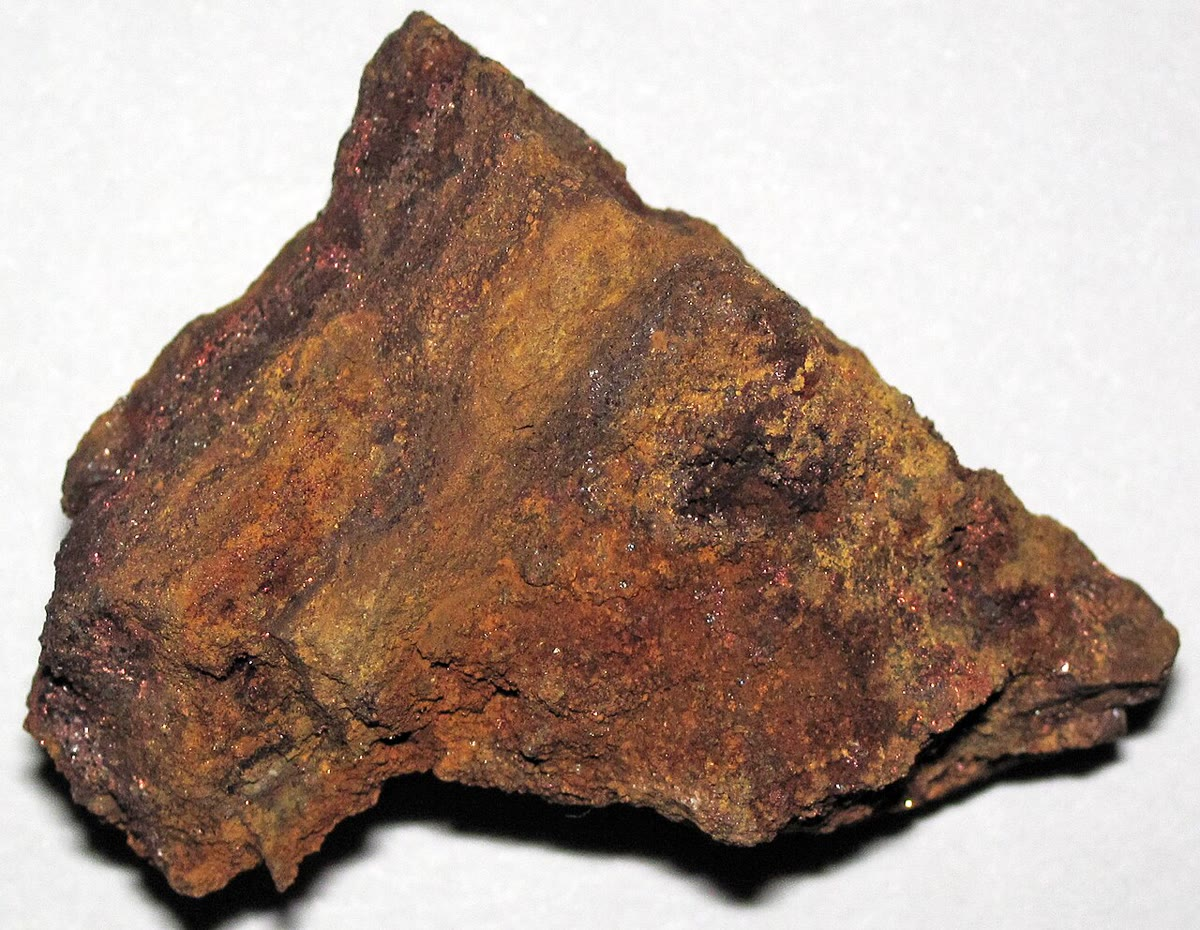
\includegraphics[width=0.4\linewidth]{images/book4/b2-29-flambeau-gossan.jpg}
\par\smallskip{\small \omterm{def:b2:ore-deposits:supergene}{Gossan} da \omterm{def:b2:ore-deposits:deposit}{jazida} de sulfeto maciço de Flambeau, Wisconsin: uma rocha porosa de
hidróxi-óxidos de ferro deixada pelo intemperismo de pirita, calcopirita, calcocita e bornita num
arco vulcânico paleoproterozoico; os pequenos pontos alaranjados são cobre nativo. Fotografia de James
St.\ John (CC BY 2.0).}
\end{omfigure}
% ledger: photo:b2-29-gossan

\section{Teor e tonelagem}\label{sec:b2:ore-deposits:grade-tonnage}

Uma compilação mundial lista 422 \omterm{def:b2:ore-deposits:hydrothermal}{jazidas de cobre pórfiro} com sua \omterm{def:b2:ore-deposits:grade}{tonelagem}, ao menor \omterm{def:b2:ore-deposits:grade}{teor de corte}
disponível, e seu \omterm{def:b2:ore-deposits:grade}{teor} médio de cobre. Um décimo delas excede \qty{1500}{Mt} e um décimo contém menos
de \qty{33}{Mt}, com uma mediana de \qty{240}{Mt}; os \omterm{def:b2:ore-deposits:grade}{teores} vão de \qty{0.24}{\percent} a
\qty{0.75}{\percent} entre os mesmos decis, com uma mediana de \qty{0.44}{\percent}. Entre os
decis a \omterm{def:b2:ore-deposits:grade}{tonelagem} espalha-se por um fator de 45, o \omterm{def:b2:ore-deposits:grade}{teor} por um fator de 3. Em eixos logarítmicos os dois histogramas aproximam-se de curvas normais, como mostra a figura abaixo:
os logaritmos da \omterm{def:b2:ore-deposits:grade}{tonelagem} têm média de 2.373 e desvio-padrão de 0.654, os do \omterm{def:b2:ore-deposits:grade}{teor}
$-0.364$ e 0.199 (logaritmos de base 10, \omterm{def:b2:ore-deposits:grade}{tonelagem} em megatoneladas, \omterm{def:b2:ore-deposits:grade}{teor} em porcentagem). O ajuste é
imperfeito: os \omterm{def:b2:ore-deposits:grade}{teores} são mais concentrados em torno do pico que uma lei lognormal, e algumas \omterm{def:b2:ore-deposits:deposit}{jazidas} de \omterm{def:b2:ore-deposits:grade}{teor} muito baixo fazem-nos
afastar-se dela num teste formal. E as duas grandezas são quase independentes, com uma correlação de
0.1 entre seus logaritmos.
% ledger: usgs08:table1, usgs08:independence, data:b4-porphyry-cu

\begin{omfigure}
\centering
\begin{minipage}[b]{0.49\linewidth}\centering
\begin{tikzpicture}
\begin{axis}[omrecord, width=0.96\linewidth, height=4.5cm, xmin=0.5, xmax=5.0, ymin=0, ymax=80,
  xlabel={tonelagem (Mt)}, ylabel={número de jazidas},
  xtick={1,2,3,4,5}, xticklabels={10,100,1000,$10^4$,$10^5$},
  tick label style={font=\scriptsize}, label style={font=\small}]
% computed in figdata/bachelor-2/ores.py part hist_t; ledger: data:b4-porphyry-cu
\addplot[ybar, bar width=0.22, fill=omDef!35, draw=omDef!70] table[x=log10_t, y=count] {figdata/out/bachelor-2-ores-hist_t.dat};
\addplot[omThm, line width=1pt, smooth] table[x=log10_t, y=fit] {figdata/out/bachelor-2-ores-hist_t.dat};
\end{axis}
\end{tikzpicture}
\end{minipage}\hfill
\begin{minipage}[b]{0.49\linewidth}\centering
\begin{tikzpicture}
\begin{axis}[omrecord, width=0.96\linewidth, height=4.5cm, xmin=-1.2, xmax=0.6, ymin=0, ymax=120,
  xlabel={teor de cobre (\%)}, ylabel={número de jazidas},
  xtick={-1,-0.69897,-0.30103,0,0.30103}, xticklabels={0.1,0.2,0.5,1,2},
  tick label style={font=\scriptsize}, label style={font=\small}]
% computed in figdata/bachelor-2/ores.py part hist_g; ledger: data:b4-porphyry-cu
\addplot[ybar, bar width=0.088, fill=omDef!35, draw=omDef!70] table[x=log10_g, y=count] {figdata/out/bachelor-2-ores-hist_g.dat};
\addplot[omThm, line width=1pt, smooth] table[x=log10_g, y=fit] {figdata/out/bachelor-2-ores-hist_g.dat};
\end{axis}
\end{tikzpicture}
\end{minipage}
\par\smallskip{\small A \omterm{def:b2:ore-deposits:grade}{tonelagem} (à esquerda) e o \omterm{def:b2:ore-deposits:grade}{teor} de cobre (à direita) das 422 \omterm{def:b2:ore-deposits:hydrothermal}{jazidas de cobre
pórfiro} da compilação mundial, em eixos logarítmicos, com as curvas normais de mesma média
e mesmo desvio-padrão em vermelho. Dados: Singer, Berger e Moring (2008), USGS.}
\end{omfigure}

\begin{proposition}[Produto de variáveis lognormais]\label{prop:b2:ore-deposits:product}
Se $\log_{10} T$ e $\log_{10} g$ são conjuntamente normais, com médias $\mu_T$ e $\mu_g$, desvios-padrão
$\sigma_T$ e $\sigma_g$ e correlação $\rho$, então o metal contido $M = Tg/100$
($g$ em porcentagem) é lognormal: $\log_{10} M$ é normal com
\begin{equation}
\mu_M = \mu_T + \mu_g - 2 , \qquad
\sigma_M^2 = \sigma_T^2 + \sigma_g^2 + 2\rho\,\sigma_T\sigma_g .
\label{eq:b2:ore-deposits:product}
\end{equation}
\end{proposition}

\begin{proof}
$\log_{10} M = \log_{10} T + \log_{10} g - 2$. Uma combinação linear de variáveis conjuntamente normais é
normal (admitido dos livros de matemática); sua média é a soma das médias e sua variância
$\operatorname{var}(X + Y) = \operatorname{var} X + \operatorname{var} Y + 2\operatorname{cov}(X, Y)$,
com $\operatorname{cov}(X, Y) = \rho\,\sigma_T\sigma_g$.
\end{proof}

Para as \omterm{def:b2:ore-deposits:deposit}{jazidas} pórfiras, $\sigma_M = \sqrt{0.654^2 + 0.199^2 + 2 \times 0.1 \times 0.654 \times
0.199} = 0.702$ e $\mu_M = 0.009$: a \omterm{def:b2:ore-deposits:deposit}{jazida} mediana contém cerca de \qty{1}{Mt} de cobre, e o
metal contido espalha-se ainda mais amplamente que a \omterm{def:b2:ore-deposits:grade}{tonelagem}. Uma lei lognormal com dispersão tão grande
põe a maior parte do metal em poucas \omterm{def:b2:ore-deposits:deposit}{jazidas}: o décimo maior contém cerca de \qty{63}{\percent} do
cobre segundo a lei, \qty{64}{\percent} nos dados (exercício~\ref{exo:b2:ore-deposits:12}). A
figura abaixo situa cada \omterm{def:b2:ore-deposits:deposit}{jazida} por sua \omterm{def:b2:ore-deposits:grade}{tonelagem} e seu \omterm{def:b2:ore-deposits:grade}{teor}, com linhas de igual cobre contido;
Bingham, com \qty{28.5}{Mt}, fica entre as linhas de 10 e de \qty{100}{Mt}.
% ledger: data:b4-porphyry-cu
% values: sd_log10_m 0.702233, mean 0.00857; median M 1.02 Mt; top 10 % share 0.631 (fit) 0.643 (data)

\begin{definition}[Curva teor--tonelagem]\label{def:b2:ore-deposits:gt}
A \emph{curva teor--tonelagem}\index{curva teor--tonelagem} de uma \omterm{def:b2:ore-deposits:deposit}{jazida} dá, como funções do
\omterm{def:b2:ore-deposits:grade}{teor de corte} $c$, a \omterm{def:b2:ore-deposits:grade}{tonelagem} $T(c)$ dos blocos com \omterm{def:b2:ore-deposits:grade}{teor} acima de $c$ e seu \omterm{def:b2:ore-deposits:grade}{teor} médio
$\bar g(c)$.
\end{definition}

\begin{proposition}[Curva teor--tonelagem de uma jazida lognormal]\label{prop:b2:ore-deposits:gt}
Se os \omterm{def:b2:ore-deposits:grade}{teores} dos blocos de uma \omterm{def:b2:ore-deposits:deposit}{jazida} de \omterm{def:b2:ore-deposits:grade}{tonelagem} total $T_0$ são lognormais, com $\ln g$ normal
de média $\mu$ (o \omterm{def:b2:ore-deposits:grade}{teor} mediano é $e^{\mu}$) e desvio-padrão $s$, então, com $z = (\mu -
\ln c)/s$,
\begin{equation}
T(c) = T_0\,\Phi(z), \qquad
\bar g(c) = e^{\mu + s^2/2}\,\frac{\Phi(z + s)}{\Phi(z)} ,
\label{eq:b2:ore-deposits:gt}
\end{equation}
e o metal acima do \omterm{def:b2:ore-deposits:grade}{teor de corte} é $M(c) = T_0\,e^{\mu + s^2/2}\,\Phi(z + s)$, uma fração $\Phi(z +
s)$ do total.
\end{proposition}

\begin{proof}
Escreva-se $\ln g = \mu + s u$, com $u$ normal padrão. Um bloco está acima do \omterm{def:b2:ore-deposits:grade}{teor de corte} quando $u > (\ln c -
\mu)/s = -z$, o que tem probabilidade $1 - \Phi(-z) = \Phi(z)$; daí $T(c)$. O metal acima do
\omterm{def:b2:ore-deposits:grade}{teor de corte} por unidade de \omterm{def:b2:ore-deposits:grade}{tonelagem} total é $\int_{-z}^{\infty} e^{\mu + s u}\,\varphi(u)\,\mathrm{d}u$,
com $\varphi$ a densidade normal padrão. Completando o quadrado, $e^{su}\varphi(u) =
e^{s^2/2}\varphi(u - s)$, de modo que a integral vale $e^{\mu + s^2/2}\,[1 - \Phi(-z - s)] = e^{\mu +
s^2/2}\,\Phi(z + s)$. Dividindo por $\Phi(z)$ obtém-se o \omterm{def:b2:ore-deposits:grade}{teor} médio.
\end{proof}

Para $c \to 0$ toda a \omterm{def:b2:ore-deposits:deposit}{jazida} é mantida, com o \omterm{def:b2:ore-deposits:grade}{teor} médio $e^{\mu + s^2/2}$, que está acima da
mediana. Elevar o \omterm{def:b2:ore-deposits:grade}{teor de corte} remove \omterm{def:b2:ore-deposits:grade}{tonelagem} mais depressa que metal, porque os blocos removidos são os
mais pobres: na \omterm{def:b2:ore-deposits:deposit}{jazida} ilustrativa da figura, elevar o \omterm{def:b2:ore-deposits:grade}{teor de corte} de 0.2 para
\qty{0.5}{\percent} mantém \qty{41}{\percent} da \omterm{def:b2:ore-deposits:grade}{tonelagem} mas \qty{61}{\percent} do cobre.
% values: demo T 876.0/355.0 Mt, M 4.599/2.826 Mt (figdata ores.py gtcurve)

\begin{omfigure}
\centering
\begin{minipage}[b]{0.49\linewidth}\centering
\begin{tikzpicture}
\begin{axis}[omrecord, width=0.96\linewidth, height=5.0cm, xmode=log, ymode=log,
  xmin=2, xmax=50000, ymin=0.05, ymax=2.8, xlabel={tonelagem (Mt)}, ylabel={teor de cobre (\%)},
  ytick={0.1,0.2,0.5,1,2}, yticklabels={0.1,0.2,0.5,1,2},
  tick label style={font=\scriptsize}, label style={font=\small}]
% computed in figdata/bachelor-2/ores.py parts scatter and iso; ledger: data:b4-porphyry-cu
\addplot[black!45, line width=0.6pt, unbounded coords=jump] table[x=tonnage_mt, y=g01] {figdata/out/bachelor-2-ores-iso.dat};
\addplot[black!45, line width=0.6pt, unbounded coords=jump] table[x=tonnage_mt, y=g1] {figdata/out/bachelor-2-ores-iso.dat};
\addplot[black!45, line width=0.6pt, unbounded coords=jump] table[x=tonnage_mt, y=g10] {figdata/out/bachelor-2-ores-iso.dat};
\addplot[black!45, line width=0.6pt, unbounded coords=jump] table[x=tonnage_mt, y=g100] {figdata/out/bachelor-2-ores-iso.dat};
\addplot[omDef, only marks, mark=*, mark size=0.8pt, opacity=0.7] table[x=tonnage_mt, y=cu_pct] {figdata/out/bachelor-2-ores-scatter.dat};
\addplot[omThm, only marks, mark=square*, mark size=2pt] coordinates {(3230,0.882)};
\node[font=\tiny, text=black!70, fill=white, inner sep=1pt] at (axis cs:4.55,2.2) {0.1};
\node[font=\tiny, text=black!70, fill=white, inner sep=1pt] at (axis cs:45.5,2.2) {1};
\node[font=\tiny, text=black!70, fill=white, inner sep=1pt] at (axis cs:455,2.2) {10};
\node[font=\tiny, text=black!70, fill=white, inner sep=1pt] at (axis cs:4545,2.2) {100 Mt};
\node[font=\scriptsize, text=omThm, anchor=south, fill=white, inner sep=1pt] at (axis cs:3230,1.0) {Bingham};
\end{axis}
\end{tikzpicture}
\end{minipage}\hfill
\begin{minipage}[b]{0.49\linewidth}\centering
\begin{tikzpicture}
\begin{axis}[omrecord, width=0.80\linewidth, height=5.0cm, xmin=0, xmax=1.2, ymin=0, ymax=1000,
  xlabel={teor de corte (\%)}, ylabel={tonelagem acima do corte (Mt)}, axis y line*=left,
  ylabel style={text=omDef}, tick label style={font=\scriptsize}, label style={font=\small}]
% computed in figdata/bachelor-2/ores.py part gtcurve (illustrative deposit)
\addplot[omDef, line width=1.1pt] table[x=cutoff_pct, y=tonnage_mt] {figdata/out/bachelor-2-ores-gtcurve.dat};
\end{axis}
\begin{axis}[width=0.80\linewidth, height=5.0cm, xmin=0, xmax=1.2, ymin=0, ymax=1.6,
  axis y line*=right, axis x line=none, ylabel={teor médio acima do corte (\%)},
  ylabel style={text=omThm}, tick label style={font=\scriptsize}, label style={font=\small}]
\addplot[omThm, line width=1.1pt, densely dashed] table[x=cutoff_pct, y=grade_pct] {figdata/out/bachelor-2-ores-gtcurve.dat};
\end{axis}
\end{tikzpicture}
\end{minipage}
\par\smallskip{\small À esquerda: \omterm{def:b2:ore-deposits:grade}{tonelagem} e \omterm{def:b2:ore-deposits:grade}{teor} de cobre das 422 \omterm{def:b2:ore-deposits:hydrothermal}{jazidas de cobre pórfiro}, com
linhas de igual cobre contido (0.1 a \qty{100}{Mt}); o quadrado vermelho é Bingham Canyon. Dados:
Singer, Berger e Moring (2008), USGS. À direita: a \omterm{def:b2:ore-deposits:gt}{curva teor--tonelagem} de uma \omterm{def:b2:ore-deposits:deposit}{jazida} ilustrativa
de \qty{1000}{Mt}, \omterm{def:b2:ore-deposits:grade}{teor} mediano \qty{0.40}{\percent}, $s = 0.60$: \omterm{def:b2:ore-deposits:grade}{tonelagem} acima do \omterm{def:b2:ore-deposits:grade}{teor de corte} (azul)
e seu \omterm{def:b2:ore-deposits:grade}{teor} médio (vermelho, tracejado), segundo \eqref{eq:b2:ore-deposits:gt}.}
\end{omfigure}

\section{A prospecção}\label{sec:b2:ore-deposits:exploration}

As \omterm{def:b2:ore-deposits:deposit}{jazidas} são encontradas pelos vestígios que deixam além de seu minério. O halo de alteração de um sistema
pórfiro tem quilômetros de largura, e onde a rocha aflora seus minerais podem ser mapeados a partir de aviões
e satélites por seus espectros infravermelhos; seus metais dispersam-se nos solos, nos sedimentos de corrente, nas águas e nas plantas em
volta; e seus sulfetos e rochas alteradas mudam as propriedades físicas que a geofísica mede.
% ledger: usgs10b:form, usgs10b:exploration, usgs10b:remote

\begin{definition}[Anomalia geoquímica]\label{def:b2:ore-deposits:exploration}
Uma \emph{anomalia geoquímica}\index{anomalia geoquímica} é uma concentração de um elemento, ou de um
grupo de elementos, num meio amostrado --- rocha, solo, sedimento de corrente, água, plantas --- que
se afasta de seu fundo regional, a faixa de concentrações encontrada onde nenhuma
mineralização está presente.
\end{definition}

Como os \omterm{def:b2:ore-deposits:grade}{teores}, as concentrações espalham-se por ordens de grandeza, de modo que uma anomalia é em geral julgada em
logaritmos; um limiar simples, usado no exercício~\ref{exo:b2:ore-deposits:9}, é a média dos
logaritmos do fundo mais duas vezes seu desvio-padrão. Uma amostra de sedimento de corrente
mistura o sedimento de toda a sua bacia, de modo que uma anomalia se atenua a jusante à medida que sedimento limpo se
junta a ela, e o gradiente das concentrações aponta rio acima, em direção à fonte. Em solos sobre
pegmatitos soterrados, anomalias de lítio, rubídio, césio, tântalo e estanho foram rastreadas acima de
corpos que não afloram.
% ledger: usgs10b:exploration, usgs10o:lct

Os métodos geofísicos são escolhidos pelo contraste que um \omterm{def:b2:ore-deposits:types}{tipo de jazida} oferece. Os sulfetos disseminados fazem uma
rocha agir como um capacitor: o método de polarização induzida, que mede essa cargabilidade, foi
desenvolvido para o cobre pórfiro e responde sobretudo à zona sericítica rica em pirita, sendo o núcleo
potássico mais pobre em sulfetos. Os levantamentos magnéticos e gravimétricos mapeiam os \omterm{def:b2:magma-emplacement:bodies}{plútons} aos quais as \omterm{def:b2:ore-deposits:deposit}{jazidas}
estão relacionadas. Nenhum método vê o minério
diretamente, e toda interpretação é não única até que um furo de sondagem a teste.
% ledger: usgs10b:exploration

\begin{method}[Das análises a uma estimativa de recursos]\label{met:b2:ore-deposits:resource}
Os dados são furos de sondagem numa malha através da \omterm{def:b2:ore-deposits:deposit}{jazida}, com seus testemunhos descritos e analisados em intervalos
de comprimento conhecido.
\begin{enumerate}
  \item \textbf{Compostas.} Faça a média das análises sobre comprimentos iguais, ponderando cada análise por seu
        comprimento, de modo que cada amostra composta represente o mesmo volume.
  \item \textbf{Modelo.} Divida a \omterm{def:b2:ore-deposits:deposit}{jazida} em blocos e estime o \omterm{def:b2:ore-deposits:grade}{teor} de cada um a partir das
        compostas próximas, ponderando-as pela distância e pela correlação espacial dos \omterm{def:b2:ore-deposits:grade}{teores}
        (o método geoestatístico da krigagem, admitido).
  \item \textbf{Relatório.} Aplique um \omterm{def:b2:ore-deposits:grade}{teor de corte}: \omterm{def:b2:ore-deposits:grade}{tonelagem} e \omterm{def:b2:ore-deposits:grade}{teor} médio dos blocos acima dele, com a
        densidade da rocha, em cada nível de confiança permitido pelo espaçamento dos furos.
\end{enumerate}
\end{method}

\begin{inthefield}[Descrever testemunhos de sondagem]
\centering
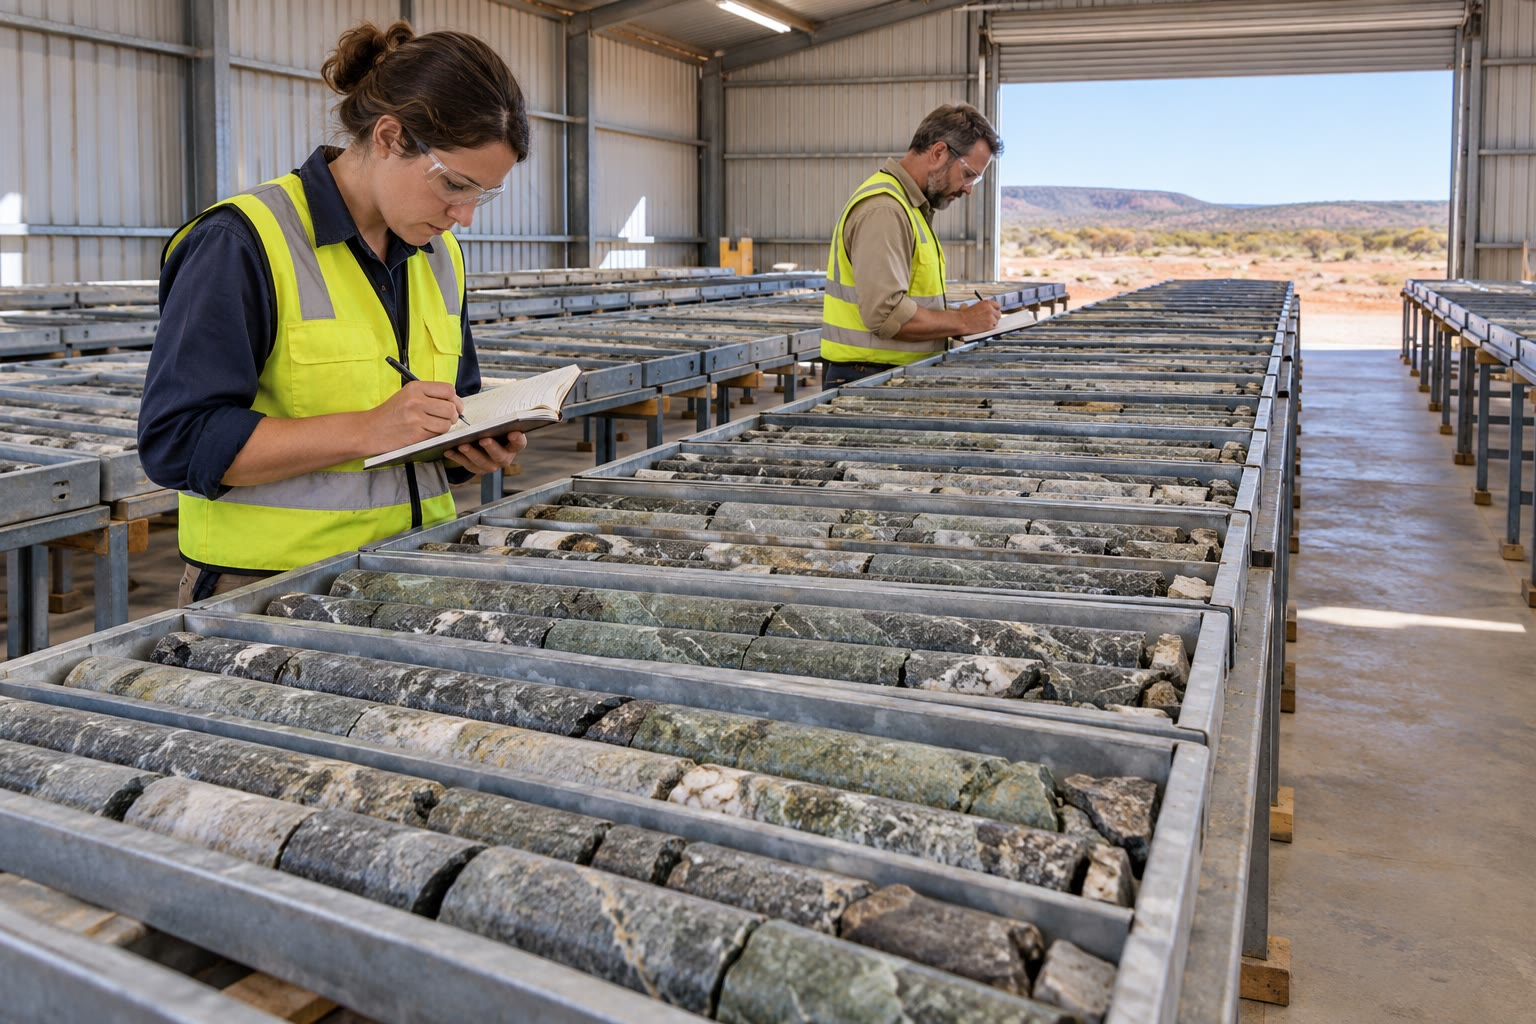
\includegraphics[width=0.56\linewidth]{images/book4/ai/b2-core-shed.jpg}
\par\smallskip{\small Um galpão de testemunhos num projeto de prospecção (ilustração gerada por IA).}
\par\medskip\raggedright
Num projeto de prospecção, os testemunhos de cada furo são dispostos em caixas metálicas na ordem
em que saíram do terreno. Os geólogos percorrem as caixas, intervalo por intervalo, e registram qual é a
rocha, como está alterada, que veios a cortam e em que proporção, e que sulfetos ela
contém; marcam onde o testemunho será serrado e amostrado. A descrição vem antes das análises e é
comparada com elas: uma zona de alteração ou um tipo de veio que carrega o metal torna-se a coisa a
seguir de furo em furo, e a partir da descrição os geólogos traçam as seções com as quais os próximos
furos são planejados.
\end{inthefield}

\section*{Exercícios}\label{sec:b2:ore-deposits:exercises}

Dados para os exercícios, salvo indicação em contrário: crosta continental superior, cobre \qty{28}{ppm},
ouro \qty{1.5}{ng/g}, cromo \qty{92}{ppm}; a população de cobres pórfiros da
\cref{sec:b2:ore-deposits:grade-tonnage}, $\log_{10}$ da \omterm{def:b2:ore-deposits:grade}{tonelagem} (Mt) com média 2.373 e desvio-padrão
0.654, $\log_{10}$ do \omterm{def:b2:ore-deposits:grade}{teor} (\%) com média $-0.364$ e desvio-padrão 0.199, correlação
$\rho = 0.100$. Arredonde a três algarismos significativos.
% ledger: rg03:ucc-trace, data:b4-porphyry-cu

\begin{exercise}[$\star$]\label{exo:b2:ore-deposits:1}
Encontre o \omterm{def:b2:ore-deposits:cf}{fator de concentração} em relação à crosta superior de: (a) um minério de cobre a
\qty{0.5}{\percent}; (b) um minério de ouro a \qty{6}{g/t}; (c) um cromitito com \qty{90}{\percent}
de cromita, tomando a cromita como FeCr$_2$O$_4$ (massas atômicas Cr 52.00, Fe 55.85, O 16.00).
\end{exercise}

\begin{exercise}[$\star$]\label{exo:b2:ore-deposits:2}
Batu Hijau é declarada com \qty{914}{Mt} a \qty{0.53}{\percent} de Cu e \qty{0.40}{g/t} de Au acima de um
\omterm{def:b2:ore-deposits:grade}{teor de corte} de \qty{0.3}{\percent}, e com \qty{1640}{Mt} a \qty{0.44}{\percent} de Cu e \qty{0.45}{g/t}
de Au ao menor \omterm{def:b2:ore-deposits:grade}{teor de corte} disponível. (a) Encontre o cobre contido (Mt) e o ouro (t) de cada
estimativa. (b) Que \omterm{def:b2:ore-deposits:grade}{tonelagem} e que cobre os blocos adicionais da segunda estimativa acrescentam, e com
que \omterm{def:b2:ore-deposits:grade}{teor} médio? (c) Por que as duas estimativas estão corretas?
\end{exercise}

\begin{exercise}[$\star$]\label{exo:b2:ore-deposits:3}
Na lei de Stokes a velocidade de sedimentação de um grão de diâmetro $d$ é proporcional a $(\rho_s -
\rho_w)\,d^2$. Tome $\rho_w = 1.00$, quartzo 2.65, ouro 19.3, zircão 4.7 (em
\unit{g.cm^{-3}}). (a) Quantas vezes mais depressa um grão de ouro sedimenta que um grão de quartzo do
mesmo tamanho? (b) Qual é a razão entre os diâmetros de um grão de ouro e de um de quartzo que sedimentam à
mesma velocidade? (c) Que grão de quartzo sedimenta como um grão de zircão de \qty{0.1}{mm}?
\end{exercise}

\begin{exercise}[$\star$]\label{exo:b2:ore-deposits:4}
Um minério primário de cobre tem um \omterm{def:b2:ore-deposits:grade}{teor} de \qty{0.4}{\percent}. O intemperismo lixivia todo o seu cobre numa
espessura de \qty{150}{m} e redeposita-o num manto de \qty{50}{m} de espessura logo abaixo, sendo a densidade
a mesma. (a) Encontre o \omterm{def:b2:ore-deposits:grade}{teor} do manto. (b) O mesmo se apenas \qty{80}{\percent} do
cobre lixiviado for redepositado. (c) Que espessura lixiviada daria \qty{1.7}{\percent} com
redeposição completa?
\end{exercise}

\begin{exercise}[$\star\star$]\label{exo:b2:ore-deposits:5}
Um \omterm{def:b2:magma-emplacement:magma}{magma} contém \qty{10}{ppb} de platina e \qty{200}{ppm} de níquel; tome $D_{\mathrm{Pt}} =
10^4$ e $D_{\mathrm{Ni}} = 500$. (a) Usando \eqref{eq:b2:ore-deposits:r-factor}, encontre os \omterm{def:b2:ore-deposits:grade}{teores} de
platina (ppm) e de níquel (\% em massa) do sulfeto para $R = 100$, \num{1000}, \num{10000}
e \num{100000}. (b) Encontre seus limites para $R \to \infty$. (c) Explique por que um minério de níquel diz
pouco sobre $R$, e um minério de platina muito.
\end{exercise}

\begin{exercise}[$\star\star$]\label{exo:b2:ore-deposits:6}
Usando \eqref{eq:b2:ore-deposits:product} para a população de cobres pórfiros: (a) encontre a média e o
desvio-padrão de $\log_{10} M$, e o cobre contido mediano. (b) Que fração das \omterm{def:b2:ore-deposits:deposit}{jazidas}
contém mais de \qty{10}{Mt} de cobre? Quantas das 422? (c) Refaça (b) ignorando a correlação.
\end{exercise}

\begin{exercise}[$\star\star$]\label{exo:b2:ore-deposits:7}
Para a \omterm{def:b2:ore-deposits:deposit}{jazida} ilustrativa da figura ($T_0 = \qty{1000}{Mt}$, mediana \qty{0.40}{\percent},
$s = 0.60$), use \eqref{eq:b2:ore-deposits:gt} para encontrar a \omterm{def:b2:ore-deposits:grade}{tonelagem}, o \omterm{def:b2:ore-deposits:grade}{teor} médio e o cobre contido
acima de \omterm{def:b2:ore-deposits:grade}{teores de corte} de \qty{0.3}{\percent} e \qty{0.6}{\percent}. Verifique um ponto na figura.
\end{exercise}

\begin{exercise}[$\star\star$]\label{exo:b2:ore-deposits:8}
Uma \omterm{def:b2:ore-deposits:deposit}{jazida} pórfira contém \qty{5}{Mt} de cobre. Suponha que seu fluido magmático transportasse \qty{1000}{ppm}
de cobre, metade do qual tenha sido depositada no minério, e que o \omterm{def:b2:magma-emplacement:magma}{magma} tenha liberado \qty{3.5}{\percent}
de sua massa como fluido. (a) Encontre a massa de fluido e de \omterm{def:b2:magma-emplacement:magma}{magma} necessária. (b) Encontre o volume do
\omterm{def:b2:magma-emplacement:magma}{magma}, de densidade \qty{2600}{kg.m^{-3}}. (c) Se o \omterm{def:b2:magma-emplacement:magma}{magma} continha \qty{50}{ppm} de cobre, que fração
dele terminou no minério?
\end{exercise}

\begin{exercise}[$\star\star$]\label{exo:b2:ore-deposits:9}
Oito sedimentos de corrente de fundo dão $\log_{10}$ Cu (ppm) de 1.30, 1.45, 1.38, 1.52, 1.41, 1.35,
1.48 e 1.40. (a) Encontre a média e o desvio-padrão (populacional) dos logaritmos, a
mediana de fundo e o limiar média mais dois desvios-padrão, em ppm. (b) Um afluente
que drena \qty{4}{km^2} de terreno mineralizado transporta sedimento a \qty{400}{ppm}; ele se junta a uma corrente que
drena \qty{36}{km^2} com a mediana de fundo. Supondo que cada quilômetro quadrado forneça a mesma
massa de sedimento, o sedimento misturado é anômalo? (c) Até que área total de bacia a
anomalia permanece acima do limiar?
\end{exercise}

\begin{exercise}[$\star\star\star$]\label{exo:b2:ore-deposits:10}
(a) Prove que $e^{su}\varphi(u) = e^{s^2/2}\varphi(u - s)$. (b) Deduza a média de uma variável
lognormal, $e^{\mu + s^2/2}$. (c) Mostre que a fração do metal acima do \omterm{def:b2:ore-deposits:grade}{teor de corte},
$\Phi(z + s)$, sempre excede a fração da \omterm{def:b2:ore-deposits:grade}{tonelagem}, $\Phi(z)$, e interprete.
\end{exercise}

\begin{exercise}[$\star\star\star$]\label{exo:b2:ore-deposits:11}
(a) A partir de \eqref{eq:b2:ore-deposits:r-factor}, encontre o $R$ para o qual $C_S$ atinge uma fração $f$
de seu teto $D\,C_L$. (b) Calcule-o para $f = 0.5$ e $0.9$ com $D = 300$ (níquel) e $D =
10^4$ (platina). (c) Compare com as faixas de $R$ dos minérios de níquel--cobre e dos recifes de EGP dadas
no texto.
\end{exercise}

\begin{exercise}[$\star\star\star$]\label{exo:b2:ore-deposits:12}
(a) Para uma variável lognormal $M$ com $\ln M$ de desvio-padrão $s$, mostre que as \omterm{def:b2:ore-deposits:deposit}{jazidas} acima
do quantil de ordem $q$ contêm uma fração $\Phi\bigl(s - \Phi^{-1}(q)\bigr)$ do metal total.
(b) Calcule-a para a população de pórfiros e $q = 0.9$. (c) O mesmo para $q = 0.99$; compare com
as quatro maiores \omterm{def:b2:ore-deposits:deposit}{jazidas}, que contêm \qty{26.6}{\percent} do cobre da compilação.
\end{exercise}
% ledger: data:b4-porphyry-cu

\begin{problem}[{Problema de fim de semana --- um prospecto pórfiro}]\label{pb:b2:ore-deposits:1}
Um prospecto pórfiro (inventado) foi sondado. Seu furo de descoberta cortou oito intervalos, de cima
para baixo (comprimento em metros, \omterm{def:b2:ore-deposits:grade}{teor} de cobre em porcentagem): 30 m a 0.12; 40 a 0.35; 50 a 0.62; 60
a 0.48; 40 a 0.27; 30 a 0.81; 50 a 0.41; 30 a 0.18. Um estudo geoestatístico de todos os furos
conclui que os \omterm{def:b2:ore-deposits:grade}{teores} dos blocos são lognormais, com mediana \qty{0.38}{\percent} e $s = 0.55$ para
$\ln g$. O corpo mineralizado é próximo de um cilindro vertical de raio \qty{450}{m} e altura
\qty{700}{m}, de densidade \qty{2.7}{t.m^{-3}}. Use os dados dos exercícios, e arredonde a três
algarismos significativos (as probabilidades a quatro).

\noindent\textbf{Parte I --- O furo de descoberta.}
\begin{enumerate}
  \item Encontre o comprimento amostrado do furo e seu \omterm{def:b2:ore-deposits:grade}{teor} médio ponderado pelo comprimento.
  \item Encontre a média aritmética dos oito \omterm{def:b2:ore-deposits:grade}{teores}. Por que a média ponderada é a correta?
  \item Que fração do comprimento está acima de \qty{0.3}{\percent}, e com que \omterm{def:b2:ore-deposits:grade}{teor} médio?
  \item Encontre o \omterm{def:b2:ore-deposits:cf}{fator de concentração} do \omterm{def:b2:ore-deposits:grade}{teor} médio ponderado em relação à crosta superior.
  \item O mesmo para o intervalo mais rico.
  \item Encontre o \omterm{def:b2:ore-deposits:grade}{teor} médio de todos os blocos da \omterm{def:b2:ore-deposits:deposit}{jazida}. O furo de descoberta é representativo?
\end{enumerate}

\noindent\textbf{Parte II --- A tonelagem acima do teor de corte.}
\begin{enumerate}[resume]
  \item Encontre o volume e a \omterm{def:b2:ore-deposits:grade}{tonelagem} $T_0$ do corpo; mantenha $T_0 = \qty{1200}{Mt}$.
  \item Para um \omterm{def:b2:ore-deposits:grade}{teor de corte} de \qty{0.3}{\percent}, encontre $z$ e a fração dos blocos acima dele.
  \item Encontre a \omterm{def:b2:ore-deposits:grade}{tonelagem} acima de \omterm{def:b2:ore-deposits:grade}{teores de corte} de 0.2, 0.3 e \qty{0.5}{\percent}.
  \item Encontre o \omterm{def:b2:ore-deposits:grade}{teor} médio acima do \omterm{def:b2:ore-deposits:grade}{teor de corte} de \qty{0.3}{\percent}.
  \item O mesmo acima de 0.2 e de \qty{0.5}{\percent}.
  \item Elevando o \omterm{def:b2:ore-deposits:grade}{teor de corte} de 0.3 para \qty{0.5}{\percent}: por que fatores mudam a \omterm{def:b2:ore-deposits:grade}{tonelagem} e o
        \omterm{def:b2:ore-deposits:grade}{teor} médio?
  \item Com que \omterm{def:b2:ore-deposits:grade}{teor de corte} metade da \omterm{def:b2:ore-deposits:grade}{tonelagem} é mantida, e qual é seu \omterm{def:b2:ore-deposits:grade}{teor} médio?
\end{enumerate}

\noindent\textbf{Parte III --- O prospecto entre os pórfiros do mundo.}
\begin{enumerate}[resume]
  \item Encontre o cobre contido no corpo inteiro, com seu \omterm{def:b2:ore-deposits:grade}{teor} médio.
  \item Encontre o escore padrão de sua \omterm{def:b2:ore-deposits:grade}{tonelagem} na população mundial, e seu percentil.
  \item O mesmo para seu \omterm{def:b2:ore-deposits:grade}{teor} médio.
  \item Encontre o desvio-padrão de $\log_{10} M$ com a correlação, e sem ela.
  \item Encontre o percentil de seu cobre contido.
  \item Quantas das 422 \omterm{def:b2:ore-deposits:deposit}{jazidas} se esperaria que contivessem mais cobre?
\end{enumerate}

\noindent\textbf{Parte IV --- O cobre acima do teor de corte.}
\begin{enumerate}[resume]
  \item Encontre o cobre contido acima do \omterm{def:b2:ore-deposits:grade}{teor de corte} de \qty{0.2}{\percent}.
  \item O mesmo acima de \qty{0.5}{\percent}.
  \item Que fração do cobre está acima de \qty{0.3}{\percent}, e que fração da
        \omterm{def:b2:ore-deposits:grade}{tonelagem}?
  \item Explique por que baixar o \omterm{def:b2:ore-deposits:grade}{teor de corte} abaixo de \qty{0.3}{\percent} acrescenta muita rocha e pouco
        cobre, usando as respostas às questões 9 e 20.
  \item Em resumo: quanto cobre o prospecto contém acima do \omterm{def:b2:ore-deposits:grade}{teor de corte} de \qty{0.3}{\percent}?
\end{enumerate}
\end{problem}
